\documentclass[a4paper,11pt, uplatex, dvipdfmx]{jsarticle}
\usepackage{amsmath,amsthm,amssymb,amsfonts,fancyhdr, enumerate, setspace, braket, emathEy, graphicx}

\newcommand{\ds}{\displaystyle}




\chead{10.3  練習問題解答 }
\lhead{}
\rhead{}
\cfoot{}

\pagestyle{fancy}

\begin{document}



\begin{enumerate}[(1)]

  \setlength{\itemsep}{2zh}

\item $\ds \iint_{D} \frac{dxdy}{\sqrt{1-x^2-y^2}}, \quad D=\Set{(x,y) \ \mid \ x^2+y^2<1}$

  \vspace{1zh}

  $D$ 上で $\ds \frac{1}{\sqrt{1-x^2-y^2}} >0$ なので,$D$ の1個の増加近似列に
  ついて極限を調べればよい.
  \[
    D_n = \Set{ (x,y) \ | \ x^2+y^2 \leqq \left( 1- \frac{1}{n}\right)^2} \quad (n \geqq 2)
  \]
  とすれば $\Set{ D_n}$ は $D$ の増加近似列なので,以下の極限を調べればよい.
  \[\tag{$\heartsuit$}
    \lim_{n \to \infty} \iint_{D_n} \frac{dxdy}{\sqrt{1-x^2-y^2}}
  \]
  極座標変換 $x=r\cos\theta, \; y=r\sin\theta$ によって $r\theta$ 平面の閉領域
  \[
    E_n = \Set{(r, \theta) \ \mid \ 0 \leqq r \leqq 1-\frac{1}{n}, \;
      0 \leqq \theta \leqq 2\pi}
  \]
  が $xy$ 平面の $D_n$ に変換される.極座標変換の Jacobian は $J(r,\theta)=r$ なので
  \[
    \begin{aligned}
      \iint_{D_n} \frac{dxdy}{\sqrt{1-x^2-y^2}}
      &= \iint_{E_n} \frac{|J(r, \theta)|}{\sqrt{1-r^2}} \ dr d\theta
        = \int_{0}^{2\pi} \left( \int_{0}^{1-\frac{1}{n}} \frac{r}{\sqrt{1-r^2}} \ dr \right)
        d\theta\\[1ex]
      &= \left(\int_{0}^{2\pi}d\theta\right) \left(\int_{0}^{1-\frac{1}{n}}
        \frac{r}{\sqrt{1-r^2}}\right)
        = 2\pi \left[ -\sqrt{1-r^2}\right]_{r=0}^{r=1-\frac{1}{n}}\\[1ex]
      & = 2\pi \left( 1 - \sqrt{1-\left(1-\frac{1}{n}\right)^2}\right)
        \to 2\pi \; (n \to \infty)
    \end{aligned}
  \]
  である.よって,極限 $(\heartsuit)$
  が存在したので $\ds \iint_{D} \frac{dxdy}{\sqrt{1-x^2-y^2}} = 2\pi$
  である.
  \begin{figure}[h]
    \centering
    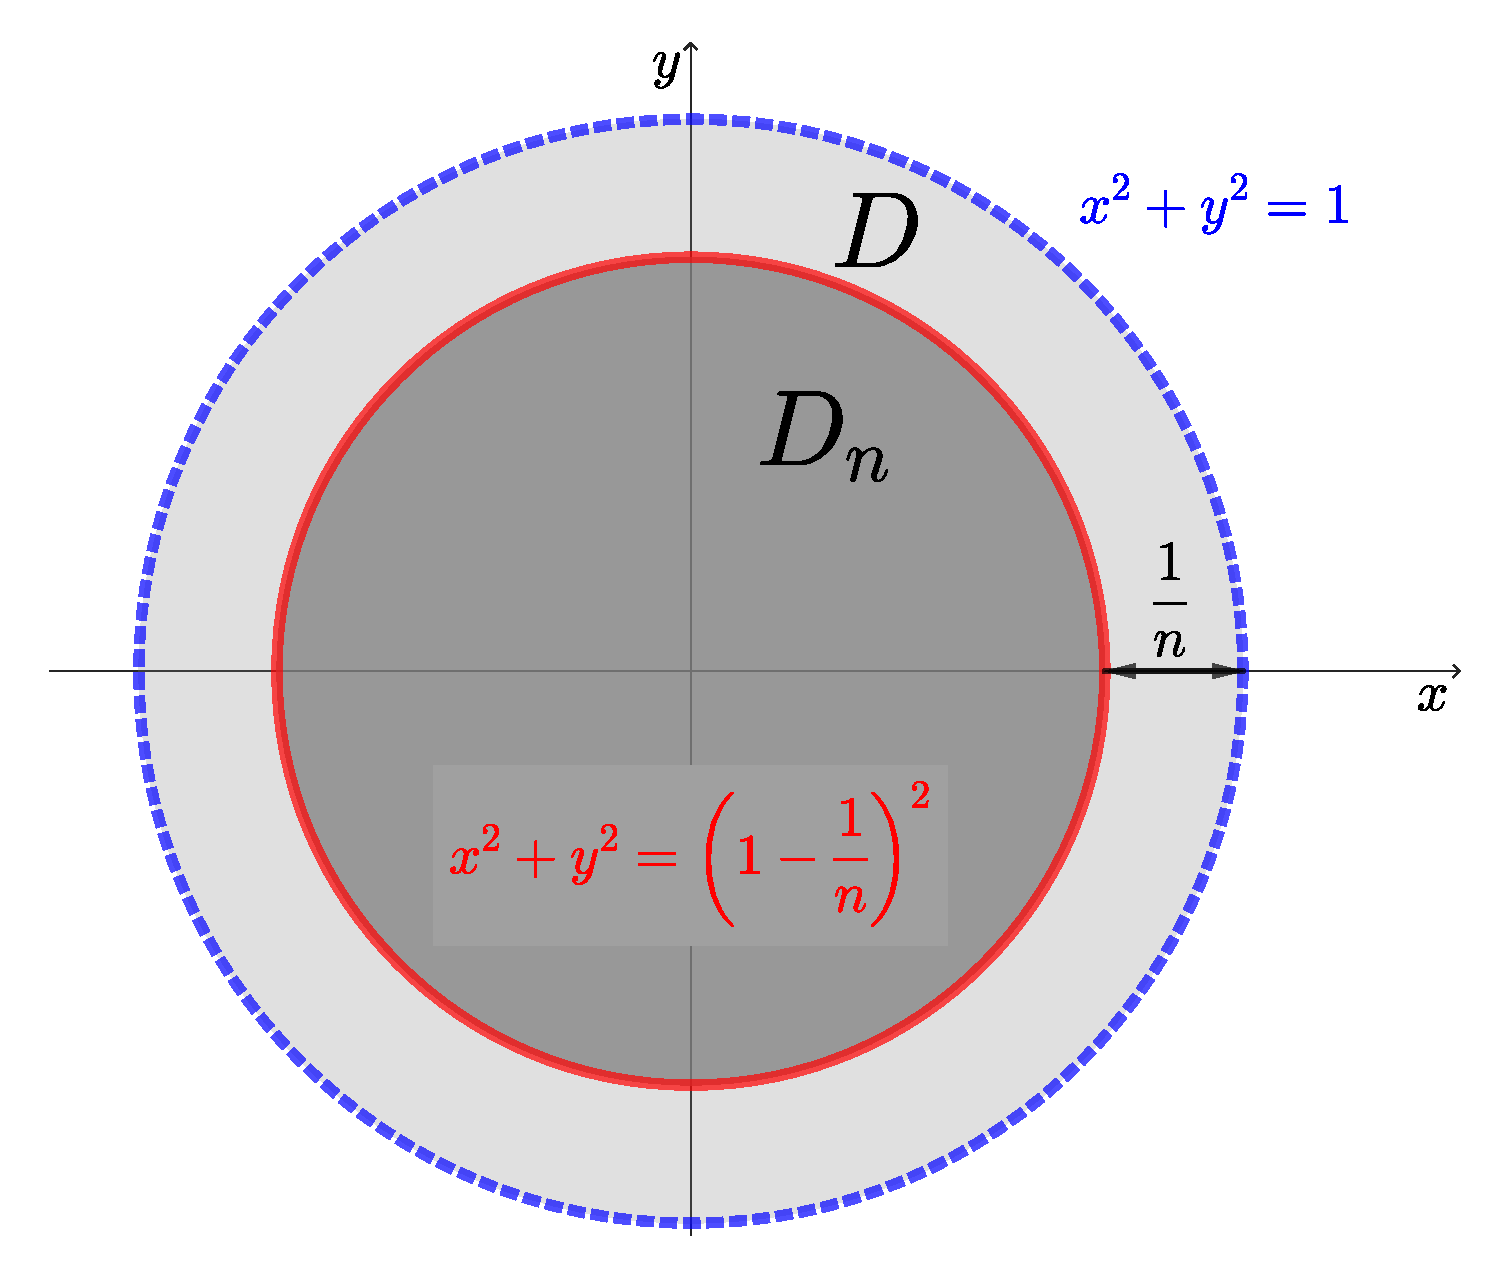
\includegraphics[height=6cm]{./pictures/D1.pdf}
  \end{figure}

  \newpage
  
\item
  $\ds \iint_{D} \frac{dxdy}{\sqrt{x^2+y^2}}, \quad D=\Set{(x,y) \
    \mid \ 0 < x \leqq 1, \; 0 \leqq y \leqq x}$

  \vspace{1zh}

  $D$ 上で $\ds \frac{1}{\sqrt{x^2+y^2}} >0 $ なので $D$ の1個の増加近
  似列について極限を調べればよい.
  \[
    D_n = \Set{(x,y) \ | \ \frac{1}{n} \leqq x \leqq 1, \; 0 \leqq
      y \leqq x} \quad (n \geqq 2)
  \]
  とすれば $\Set{D_n}$ は $D$ の増加近似列なので,以下の極限を調べればよい.
  \[\tag{$\diamondsuit$}
    \lim_{n \to \infty} \iint_{D_n} \frac{dxdy}{\sqrt{x^2+y^2}}
  \]
  $D_n$ 上の2重積分は以下のように計算できる.
  \[
    \begin{aligned}
      \iint_{D_n} \frac{dxdy}{\sqrt{x^2+y^2}}
      &= \int_{\frac{1}{n}}^{1} \left( \int_{0}^{x} \frac{dy}{\sqrt{x^2+y^2}} \right) dx
        = \int_{\frac{1}{n}}^{1} \left[ \log\left( y +
        \sqrt{x^2+y^2} \right)\right]_{y=0}^{y=x} \ dx\\[1ex]
      &=\int_{\frac{1}{n}}^{1}\left( \log\left(x+\sqrt{2x^2}\right)
        - \log \left(\sqrt{x^2}\right)\right) \ dx
        = \int_{\frac{1}{n}}^{1} \log\left(1+\sqrt{2}\right) \ dx\\[1ex]
      &= \left(1-\frac{1}{n}\right) \log \left(1+\sqrt{2}\right)
        \to \log\left(1+\sqrt{2}\right) \; (n \to \infty )
    \end{aligned}
  \]
  よって,極限 $(\diamondsuit)$ が存在したので
  $\ds \iint_{D}\frac{dxdy}{\sqrt{x^2+y^2}} =
  \log\left(1+\sqrt{2}\right)$ である.

  \begin{figure}[h]
    \centering
    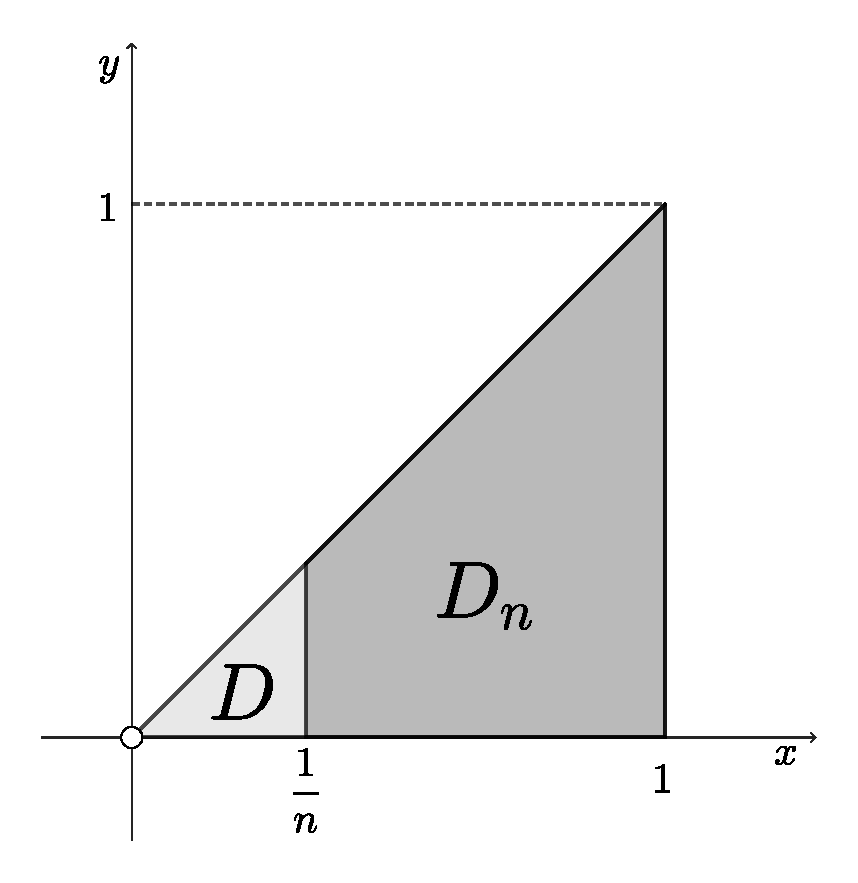
\includegraphics[height=8cm]{./pictures/D2.pdf}
  \end{figure}
  
\newpage  

\item
  $\ds \iint_{D} \tan^{-1}\frac{y}{x} \ dx dy, \quad D=\Set{(x,y) \
    \mid \ x^2+y^2 \leqq 2, \; 0 <x, \; 0 \leqq y}$


  \vspace{1zh}

  $D$ 上で $\ds \tan^{-1}{y}{x} \geqq 0$ なので,$D$ の1個の増加近似列について極限を調べればよい.
  極座標変換 $x=r\cos\theta, \; y=r\sin\theta$ によって
  \[
    E_n=\Set{(x,y) \ | \ \frac{1}{n} \leqq r \leqq \sqrt{2}, \;\; 0 \leqq \theta \leqq \frac{\pi}{2}-\frac{1}{n}} 
  \]
  が変換される $xy$ 平面の閉領域を $D_n$ とすれば,$\Set{D_n}$ は $D$ の増加近似列なので,極限
  \[
    \tag{$\clubsuit$}
    \lim_{n \to \infty} \iint_{D_n} \tan^{-1}\frac{y}{x} \ dxdy
  \]
  を調べればよい.$0\leqq \theta < \frac{\pi}{2}$ なので
  $\ds \tan^{-1}(\tan\theta) = \theta$ であり,極座標変換
  の Jacobian は $J(r,\theta)=r$ なので,
  \[
    \begin{aligned}
      \iint_{D_n} \tan^{-1}\frac{y}{x} \ dx dy
      &= \iint_{E_n} \tan^{-1}\left(\tan \theta\right) |J(r,\theta)| \ drd\theta
        = \left(\int_{0}^{\frac{\pi}{2}-\frac{1}{n}}\theta \ d\theta\right) \left( \int_{\frac{1}{n}}^{\sqrt{2}} r \ dr\right)\\[1ex]
      &= \left[ \frac{\theta^2}{2}\right]_{0}^{\frac{\pi}{2}-\frac{1}{n}} \left[\frac{r^2}{2}\right]_{\frac{1}{n}}^{\sqrt{2}}
        = \frac{1}{4}\left( \frac{\pi}{2}-\frac{1}{n}\right)^2\left( 2 - \left(\frac{1}{n}\right)^2\right)
        \to \frac{\pi^2}{8} \; (n \to \infty)
    \end{aligned}
  \]
  である.よって,極限 $(\clubsuit)$ が存在したので $\ds \iint_{D} \tan^{-1}\frac{y}{x} \ dx dy = \frac{\pi^2}{8}$ である.

  \begin{figure}[h]
    \centering
    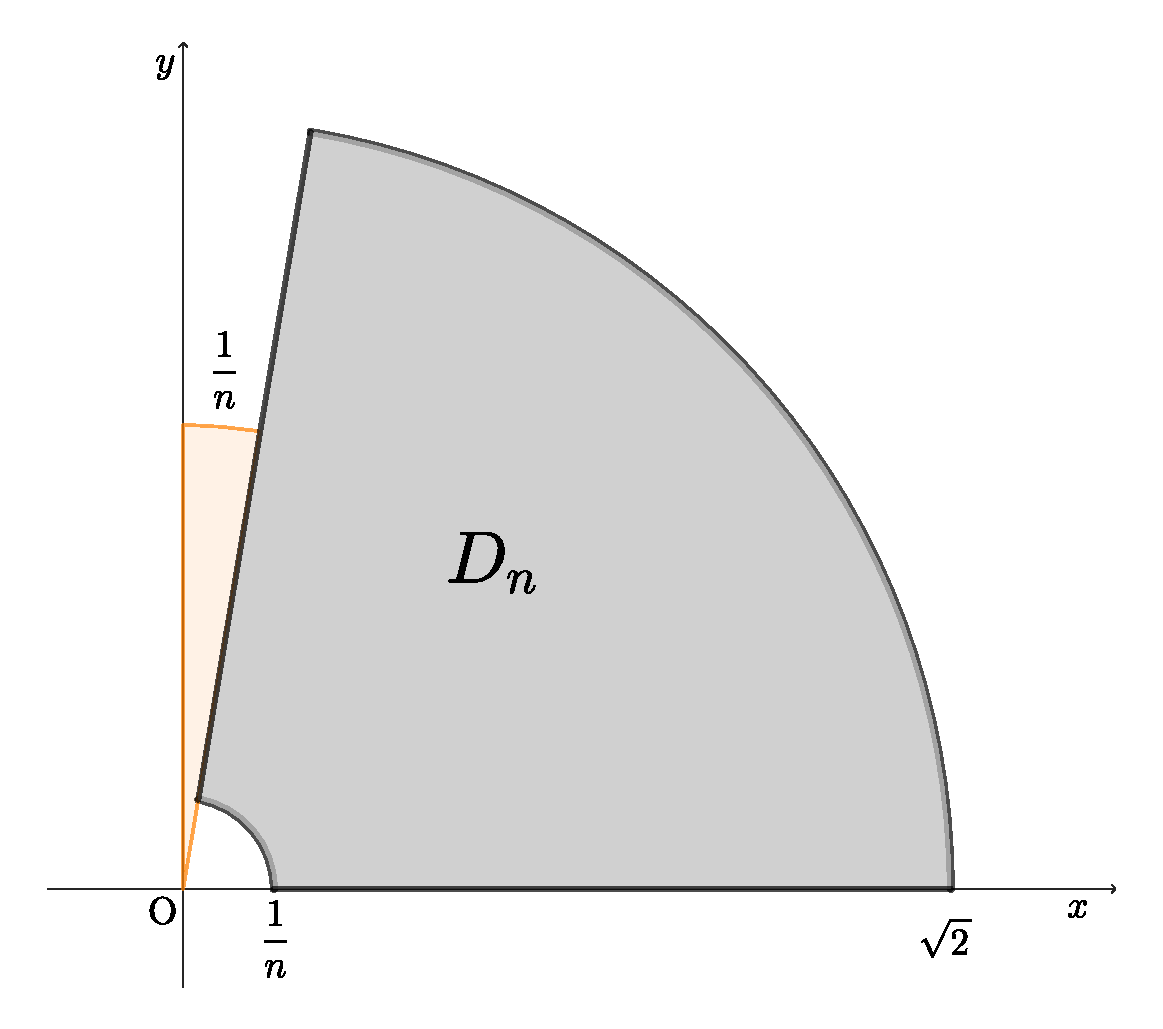
\includegraphics[height=8cm]{./pictures/D3.pdf}
  \end{figure}
\end{enumerate}



\end{document}

